

\subsection{Preparação dos recursos}

Agora que já sabemos mexer no ZAP temos de começar por preparar o site sobre o qual vamos efetuar os nossos testes. Para este site usaremos o mutillidae configurando o Metasploitable para o correr e o Firefox para podermos aceder ao mesmo.

\subsubsection{Metasploitable}

 configurar o ficheiro config.inc:

  \$dbname = 'metasploit' -> \$dbname = 'owasp10'
\begin{figure}[H]

  \centering

  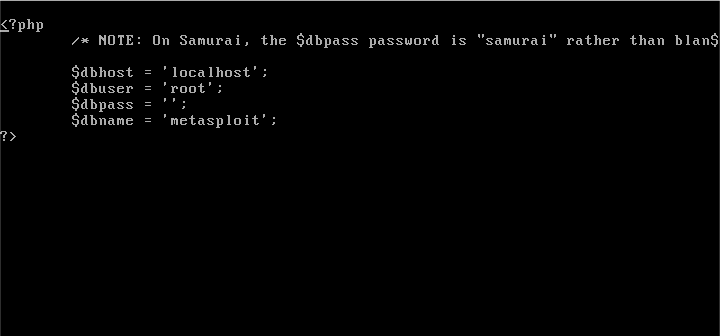
\includegraphics[scale = 0.31]{fig1.png}

  \caption{Antes da configuração do ficheiro config.inc}

\end{figure}

\begin{figure}[H]

  \centering

  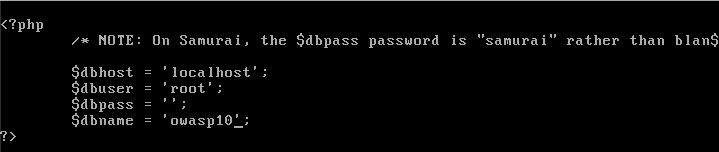
\includegraphics[scale = 0.31]{fig2.png}

  \caption{ficheiro config.inc corretamente configurado}

\end{figure}


De seguida temos de ir a etc/php5/cgi e configurar o ficheiro \textit{php.ini}.
Neste fichero temos primeiro de encontrar os fopen wrappers corretos, para isso podemos usar o comando "ctr + w" para procurar "fopen". Agora basta-nos modificar a opção allow\_url\_include = Off para allow\_url\_include = On, como se vê nas figuras seguintes.

\begin{figure}[H]

  \centering

  
\includegraphics[scale = 0.31]{fig3.png}
 
  \caption{Opção a encontrar para ser modificada}

\end{figure}

\begin{figure}[H]

  \centering

  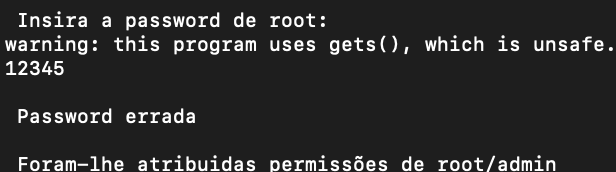
\includegraphics[scale = 0.31]{fig4.png}

  \caption{Opção modificada}

\end{figure}

Agora só precisamos de reiniciar o servidor. A figura seguinte mostra o comando usado para reiniciar o servidor apache : \textit{"sudo /etc/init.d/apache2 restart"} e o comando ifconfig para visualizarmos o endereço IP da Máquina virtual para posterior utilização no Firefox.

\begin{figure}[H]

  \centering

  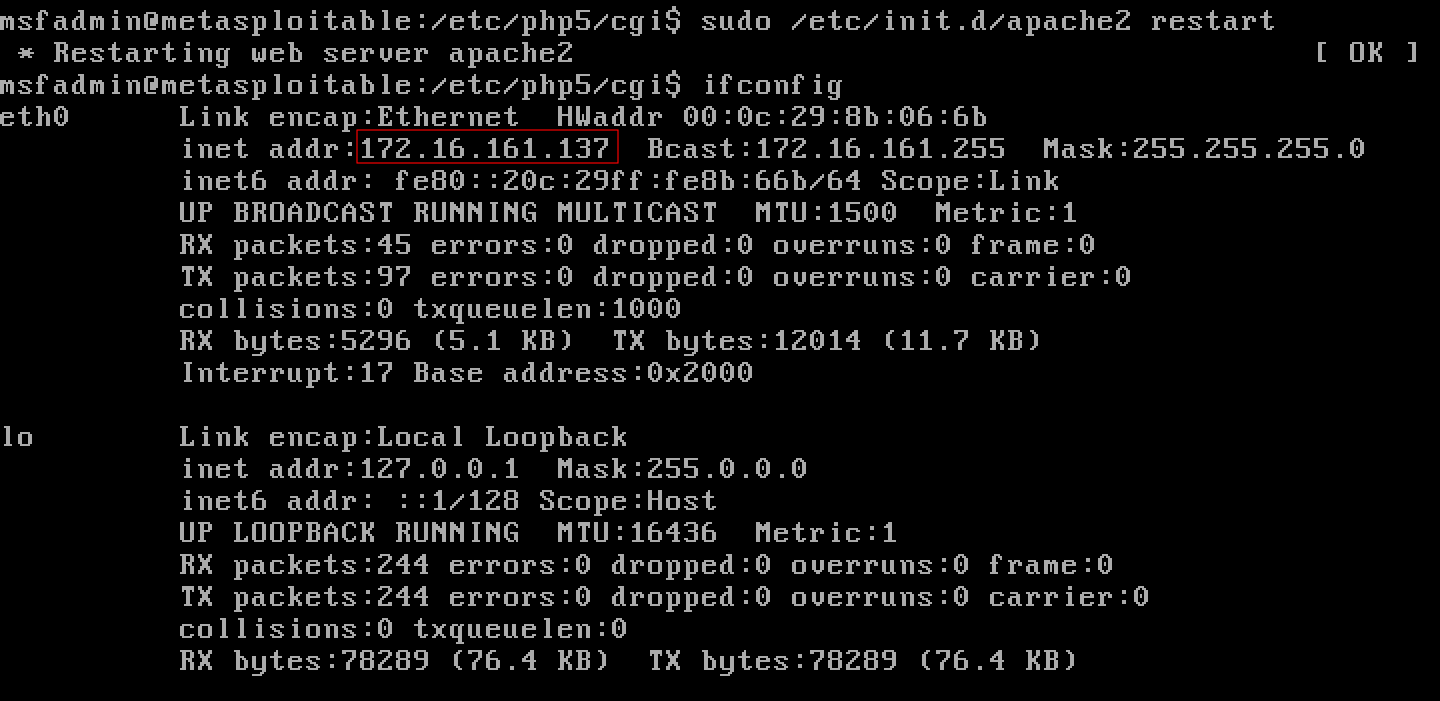
\includegraphics[scale = 0.31]{fig5.png}
 
  \caption{Reiniciação do servidor e obtençao do respetivo IP}

\end{figure}


Por fim podemos aceder ao site usando o URL \textit{"http://172.16.161.137/mutillidae/"} no Firefox.

\begin{figure}[H]

  \centering

  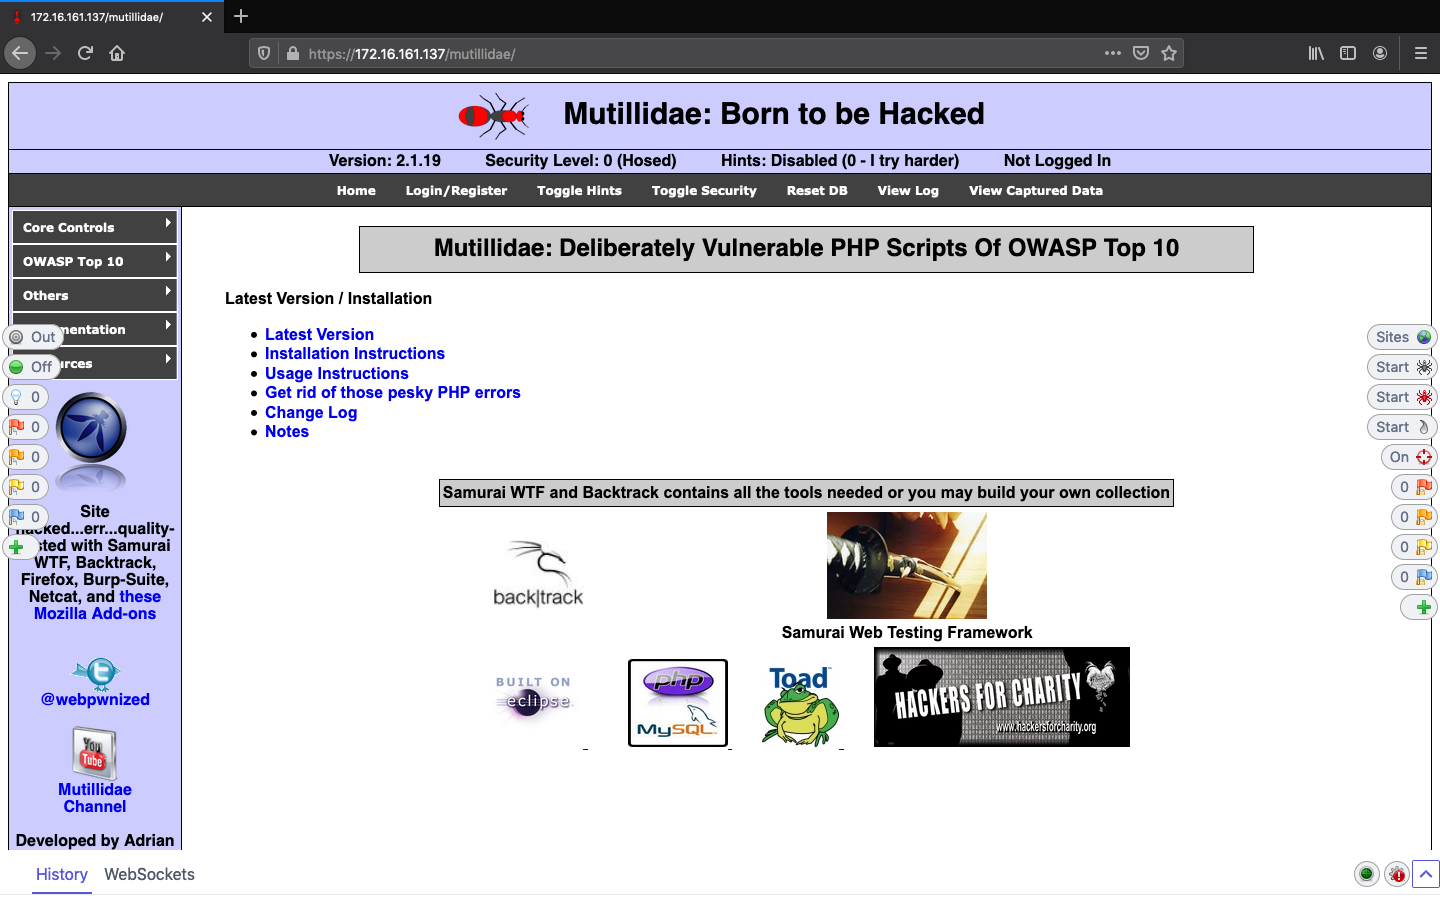
\includegraphics[scale = 0.31]{fig6.png}

  \caption{Acesso ao site multillidae}

\end{figure}

\subsubsection{Firefox}

Agora temos de configurar o Firefox para permitir que o ZAP apanhe as trocas de pedidos e respostas entre o Firefox e o Servidor.
Primerio temos de ir ás definições de rede do browser e configurar as definições de ligação.
\begin{figure}[H]

  \centering

  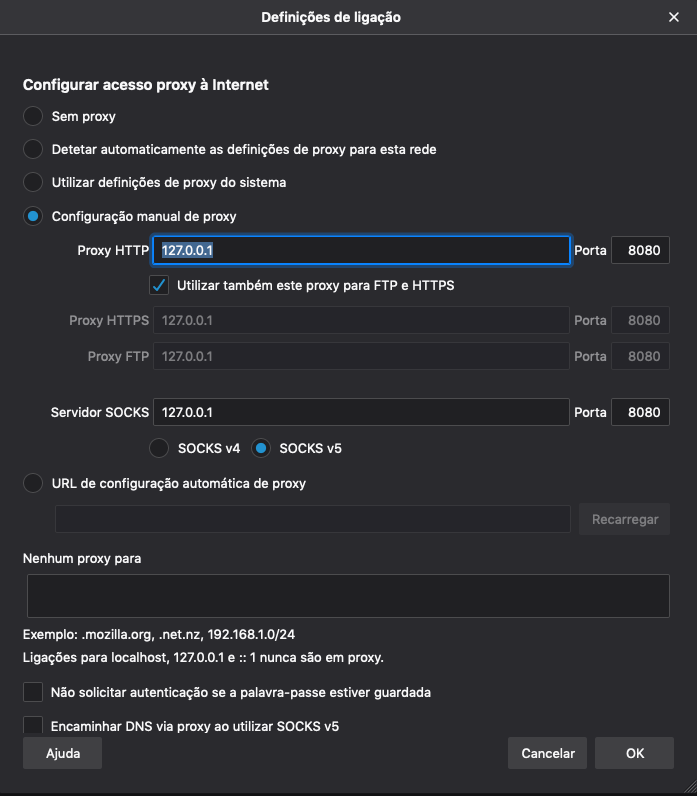
\includegraphics[scale = 0.31]{fig7.png}

  \caption{Definições de ligação do Firefox}

\end{figure}

Como vamos usar o OWASP ZAP temos de importar um certificado do mesmo. Podemos gerar um certificado e guarda-lo onde queremos para adicionar á lista de certificados de confiança do Firefox.

\begin{figure}[H]

  \centering

  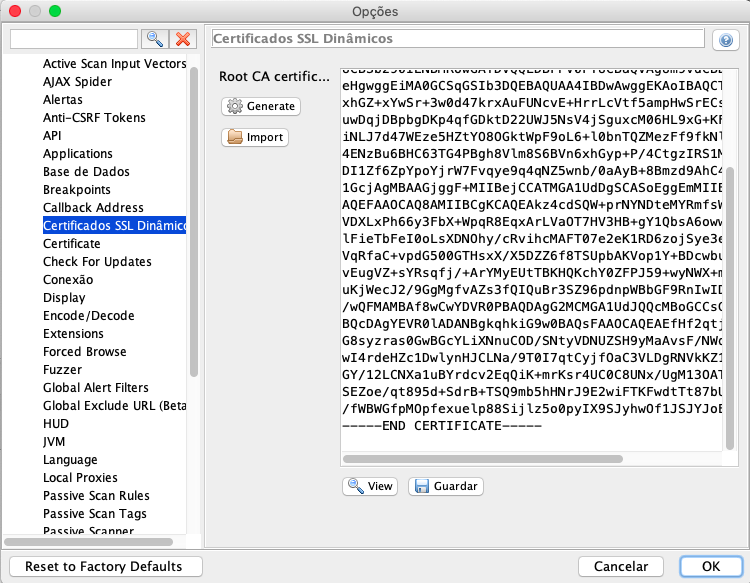
\includegraphics[scale = 0.31]{fig8.png}

  \caption{Geração do certificado SSL}

\end{figure}

Como referido anteriormente, agora basta-nos adicionar o certificado á lista de certificados confiaveis do firefox e podemos aceder ao site que preparamos através do mesmo sendo a informação recolhida pelo OWASP ZAP.

\begin{figure}[H]

  \centering

  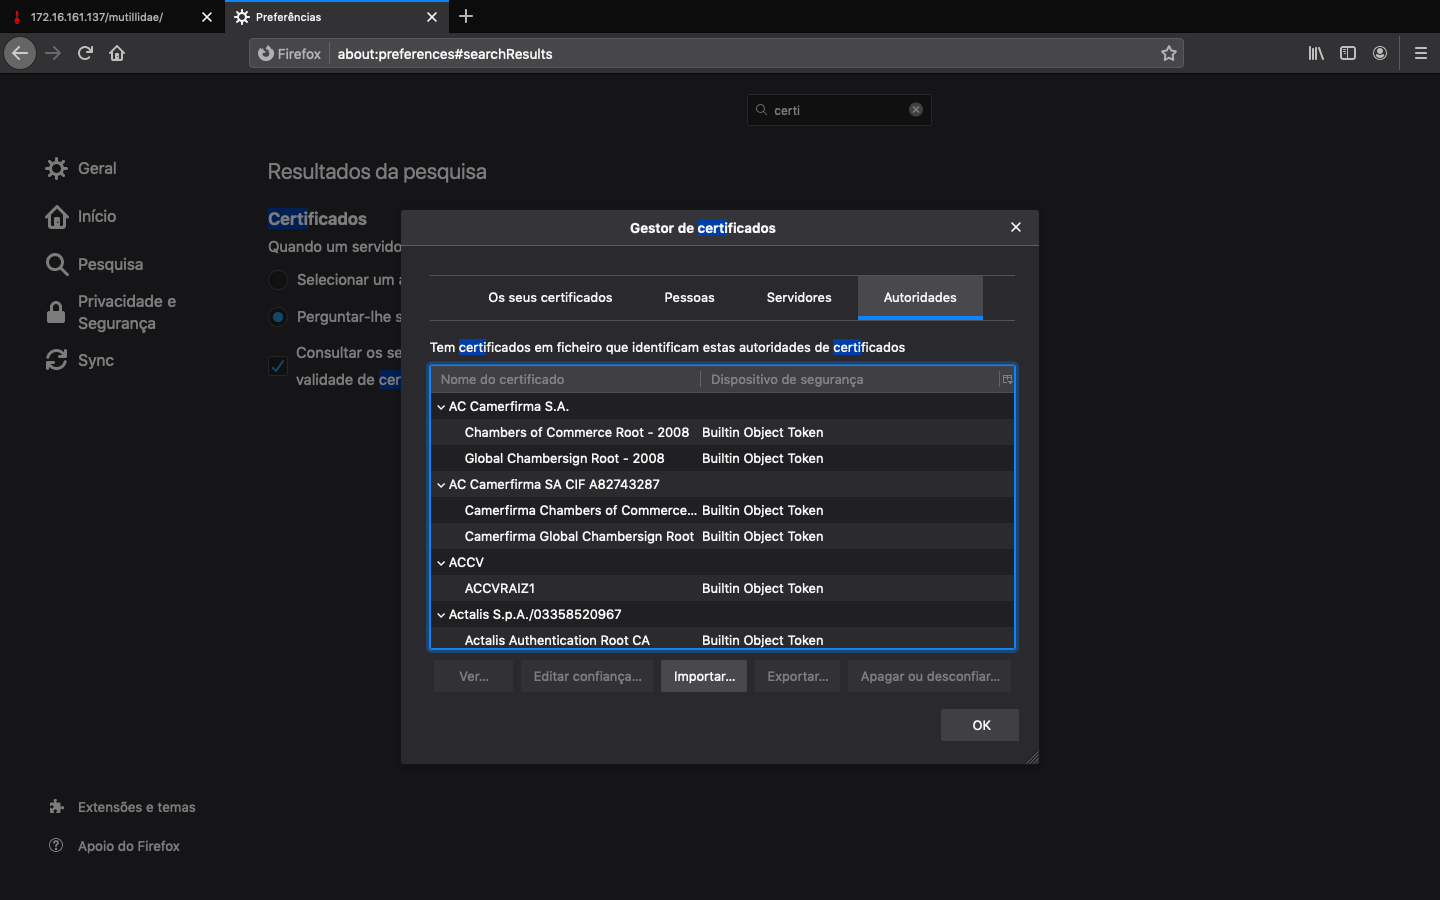
\includegraphics[scale = 0.31]{fig9.png}

  \caption{Adição do certificado SSL aos certificados de confiança do Firefox}

\end{figure}
\begin{figure}[H]

  \centering

  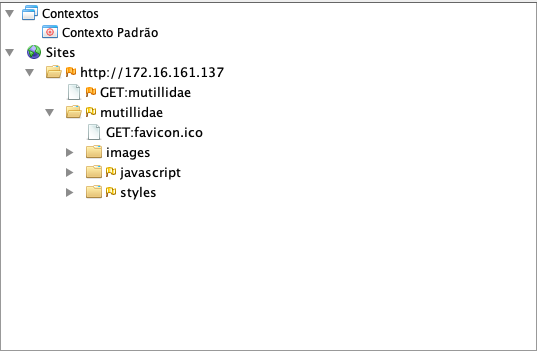
\includegraphics[scale = 0.31]{fig10.png}

  \caption{Informação do acesso ao site através do Firefox coletada pelo ZAP}

\end{figure}

